% \documentclass{beamer}
%Для защит онлайн лучше использовать разрешение 16x9
\documentclass[aspectratio=169]{beamer}

\usepackage{beamerthemesplit}
\usepackage{wrapfig}
\usetheme{SPbGU}
\usepackage{pdfpages}
\usepackage{amsmath}
\usepackage{cmap} 
\usepackage[T2A]{fontenc} 
\usepackage[utf8]{inputenc}
\usepackage[english,russian]{babel}
\usepackage{indentfirst}
\usepackage{amsmath}
\usepackage{tikz}
\usepackage{multirow}
\usepackage[noend]{algpseudocode}
\usepackage{algorithm}
\usepackage{algorithmicx}
\usetikzlibrary{shapes,arrows}
\usepackage{fancyvrb}
\usepackage{appendixnumberbeamer}

\newtheorem{rutheorem}{Теорема}
\newtheorem{ruproof}{Доказательство}
\newtheorem{rudefinition}{Определение}
\newtheorem{rulemma}{Лемма}
\usepackage{listings}
\lstdefinelanguage{NeoIDL}{
  sensitive = true,
  keywords={},
  otherkeywords={% Operators
    >, <, ==
  },
  keywords = [2]{module, resource, enum, annotation, for, import, entity, path,
  @get, @post, @put, @delete, require, ensure, otherwise, call},
  keywordstyle=\color{green},
  keywordstyle=[2]\color{blue},% for example
  numbers=left,
  numberstyle=\scriptsize,
  stepnumber=1,
  numbersep=8pt,
  showstringspaces=false,
  breaklines=true,
  frame=top,
  comment=[l]{//},
  morecomment=[s]{/*}{*/},
  commentstyle=\color{purple}\ttfamily,
  stringstyle=\color{red}\ttfamily,
  morestring=[b]',
  morestring=[b]"
  }
\lstdefinestyle{base}{
  language=C,
  emptylines=1,
  breaklines=true,
  basicstyle=\ttfamily\color{black},
  moredelim=**[is][\color{red}]{@}{@},
}
% \lstset{numbers=left, numberstyle=\tiny, stepnumber=1, numbersep=5pt,showspaces=false}


\beamertemplatenavigationsymbolsempty


% То, что в квадратных скобках, отображается внизу по центру каждого слайда. 
\title[Анализатор сетевых пакетов MimiShark]{Анализатор сетевых пакетов с веб-интерфейсом.}

% То, что в квадратных скобках, отображается в левом нижнем углу. 
\institute[СПбГУ]{}

% То, что в квадратных скобках, отображается в левом нижнем углу.
\author[Андрей Диденко]{Андрей Антонович Диденко, Б-07.21 ММ }
 
\begin{document}
{
\setbeamertemplate{footline}{}
% Лого университета или организации, отображается в шапке титульного листа
\begin{frame}
	
\includegraphics[width=1.4cm]{pictures/SPbGU_Logo.png}
	\vspace{-35pt}
	\hspace{-10pt}
	\begin{center}
		\begin{tabular}{c}
			\scriptsize{Санкт-Петербургский государственный университет} \\
			\scriptsize{Кафедра системного программирования}
		\end{tabular}
		\titlepage
	\end{center}

	\btVFill

	{\scriptsize
		% У научного руководителя должна быть указана научная степень
		{\bfseries Научный руководитель:}  И. В. Зеленчук, старший преподаватель кафедры системного программирования \\
		% Консультанта может и не быть. Должна быть указана должность или ученая степень
		% {\bfseries Консультант:}  к.ф.-м.н. Д.С.Косарев, "MatMex, JetBrains Research laboratory" \\
		% Для курсовой не обязателен. Должна быть указана должность или ученая степень
		% {\bfseries Рецензент:} д.т.н., проф. И.И. Иванов, исполнительный директор ООО ``Рога и копыта''
	}
	\begin{center}
		\vspace{5pt}
		\scriptsize{Санкт-Петербург\\
			2023}
	\end{center}

\end{frame}
}

\begin{frame}[fragile]
	\frametitle{Введение}
	\begin{itemize}
		\item Работа направлена на упрощение практической части в изучении работы компьютерных сетей
		\item Удобство (анализатор находится <<под рукой>>, не нужно пользоваться сторонними программами)
		      % Краткий обзор тематики работы (как вариант --- устно, пока показывается титульный слайд)
		\item Данное решение предназначено для студентов, изучающих предмет <<Компьютерные сети>> и связанные с ним курсы
		      % Не нужно определять общеизвестные понятия
		      % \item Сообщество miniKanren всерьез еще этим не занималось, поэтому 
		\item Визуализация пакетов для удобной работы с ними
		      % Применимость/полезность данной работы, обоснование выбора именно этой темы
		      % \item Если тема похожа на темы других работ (в том числе прошлых лет), надо явно описать разницу
	\end{itemize}
\end{frame}


\begin{frame}
	\frametitle{Постановка задачи}
	\textbf{Целью} работы является интеграция веб-интерфейса, отображающего сетевые пакеты и информацию о протоколе в Miminet.  %озвученной выше  

	\textbf{Задачи}:
	\begin{itemize}
		% \item Выбрать алгоритм, подход, метод %основываясь на проведённом анализе проблемы, области, существующих решений
		% \item Доказать корректность алгоритма
		\item Провести обзор существующих веб аналогов, предоставляющих такие же функции, как Wireshark
		      %\item Изучить примеры параллелизации
		\item На основе требований спроектировать сервис
		\item Сверстать веб-страницу
		\item Передать информацию о пакетах на страницу
		\item Внедрить реализованный сервис в Miminet
		% \footnote{\url{https://github.com/Kakadu/unicanren} (Дата доступа: 03.01.2023)}
		      % \item Подзадачи:
		      % \begin{itemize}
		      %   % \item Выбрать алгоритм, подход, метод %основываясь на проведённом анализе проблемы, области, существующих решений
		      %         % \item Доказать корректность алгоритма
		      %   \item запустить параллельно append$^{o}$
		      %   %\item Изучить примеры параллелизации
		      %   \item запустить параллельно revers$^{o}$
		      %   \item Объединить поток Stream в ответ
		      % \end{itemize}
	\end{itemize}
\end{frame}



\begin{frame}
	\frametitle{Аналоги}
	\begin{itemize}
		\item CloudShark\footnote{\url{https://www.qacafe.com/analysis-tools/cloudshark/}(Дата доступа: 15.05.22)}
		\item PacketSafari\footnote{\url{https://www.packetsafari.com/}(Дата доступа: 15.05.22)}
		\item PacketTotal\footnote{\url{https://packettotal.com/}(Дата доступа: 15.05.22)}

		      % \item Почему была выбрана 5 версия? В 4 версии нет настоящего параллелизма (приходится запускать системные потоки и параллельность происходит на уровне системы, а не на уровне OCaml)
	\end{itemize}
\end{frame}

% \begin{frame}
%   \frametitle{Используемые инструменты, подходы}
%   \begin{itemize}
%     \item За основу взят язык программирования OCaml, а также встаиваемый в него язык miniKanren
%     \item Для разработки моего проекта была задействована библиотека Domainslib для OСaml версии 5
%     \item В 5 версии добавлены новые инструменты для параллелизации 
%   \end{itemize}

% \end{frame}

% \begin{frame}
%   \frametitle{Существующие решения}
%   Возможно, предметная область сложна и потребуется больше одного слайда, но затягивать введение не стоит. Постарайтесь уложиться в 1--2 слайда
%   \begin{itemize}
%     \item Выводы
%           \begin{itemize}
%             \item Подвести итог
%             \item Указать недостатки существующих подходов, на борьбу с которыми
%                   направленна данная работа
%             \item Чётко сформулировать существующую проблему, которая будет решаться в данной работе
%           \end{itemize}
%   \end{itemize}
% \end{frame}


% Обязательный слайд: четкая формулировка цели данной работы и постановка задачи
% Описание выносимых на защиту результатов, процесса или особенностей их достижения и т.д.
%Идеально, если есть по одному слайду на каждую поставленную задачу            

\begin{frame}
	\frametitle{Используемые инструменты, подходы}
	\begin{itemize}
		\item Серверная часть была реализована с использованием фреймворка Flask\footnote{\url{https://flask.palletsprojects.com/en/2.3.x/}(Дата доступа: 15.05.22)}
		\item Чтобы создать графическую часть сервиса использовался фреймворк Bootstrap5\footnote{\url{https://getbootstrap.com/}(Дата доступа: 15.05.22)}
		\item Для работы с pcap файлами была использована библиотека dpkt\footnote{\url{https://kbandla.github.io/dpkt/}(Дата доступа: 15.05.22)} для Python
		      % \item Почему была выбрана 5 версия? В 4 версии нет настоящего параллелизма (приходится запускать системные потоки и параллельность происходит на уровне системы, а не на уровне OCaml)
	\end{itemize}
\end{frame}


% \begin{frame}
%   \frametitle{Алгоритм распараллеливания}
%   \begin{itemize}
%     \item 1.Рассматривая реализацию миниканрен на окамл,которая называется unicanren,
%           придём к выводу, что можно распараллелить функцию Conde.
%     \item При попытке параллелить функцию eval, результаты оказались отрицательным
%     \item Делаем вывод,что необходимо параллелить run. Хотим доставать ответы по мере поступаления изнутри функции и вытягивать их на верхний уровень(в ответ)
%   \end{itemize}
% \end{frame}


% \begin{frame}
%   \frametitle{DomainsLib}
%   % Задается ширина столбцов
%   \begin{itemize}
%   \item Для распараллеливания используется библиотека DomainsLib\footnote{\url{https://github.com/ocaml-multicore/parallel-programming-in-multicore-ocaml}(Дата доступа: 08.12.22)}, 
%   в которой присутствуют 2 модуля: Task -- для вызова многопоточности и Chan -- для передачи информации между доменами
%   % \item Для освоения способов применения мною были изучены предложенные примеры параллельного сложения матриц и рассмотренна реализация чисел Фибоначчи, которая тоже была распараллелена
%   \end{itemize}
% \end{frame}


% \begin{frame}[fragile]
%   \frametitle{Доказательство корректности алгоритма}
%   {\tiny Формулировки утверждений. Идеи доказательств проговариваются устно.}
%   \begin{rutheorem}[Пифагора: геометрическая формулировка]
%     В прямоугольном треугольнике площадь квадрата, построенного на гипотенузе, равна сумме площадей квадратов, построенных на катетах.
%   \end{rutheorem}

%   \begin{rutheorem}[Пифагора: алгебраическая формулировка]
%     В прямоугольном треугольнике квадрат длины гипотенузы равен сумме квадратов длин катетов.

%     То есть, если обозначить длину гипотенузы треугольника через $c$, а длины катетов
%     через $a$ и $b$, получим верное равенство: $a^2 + b^2 = c^2$.
%   \end{rutheorem}

%   \begin{rutheorem}[Обратная теорема Пифагора]
%     Для всякой тройки положительных чисел a, b и c, такой, что $a^2 + b^2 = c^2$, существует прямоугольный треугольник с катетами a и b и гипотенузой c.
%   \end{rutheorem}
% \end{frame}

% \begin{frame}
%   \frametitle{Unicanren}
%   \begin{itemize}
%   \item Вся проделанная работа выполнена на минимальной реализации miniKanren -- Unicanren\footnote{{https://github.com/Kakadu/unicanren}(Дата доступа: 08.12.22)}, которая состоит из 4 базовых конструкций: Fresh, Unify, Conde и Conj
%   % \item В этой работе есть возможность параллелить только дизъюнкцию (conde), так как это выполнение двух независимых задач, в то время как все остальное -- зависимые задачи и нет осознания того, как их параллелить

%   \end{itemize}
%   \end{frame}

% \begin{frame}[fragile]
%   \frametitle{Архитектура решения}
%   \begin{itemize}
%     \item В реализации интересны архитектура, библиотеки, инструменты
%     \item Не надо добавлять на слайд примеры кода
%   \end{itemize}
%   \begin{center}
%     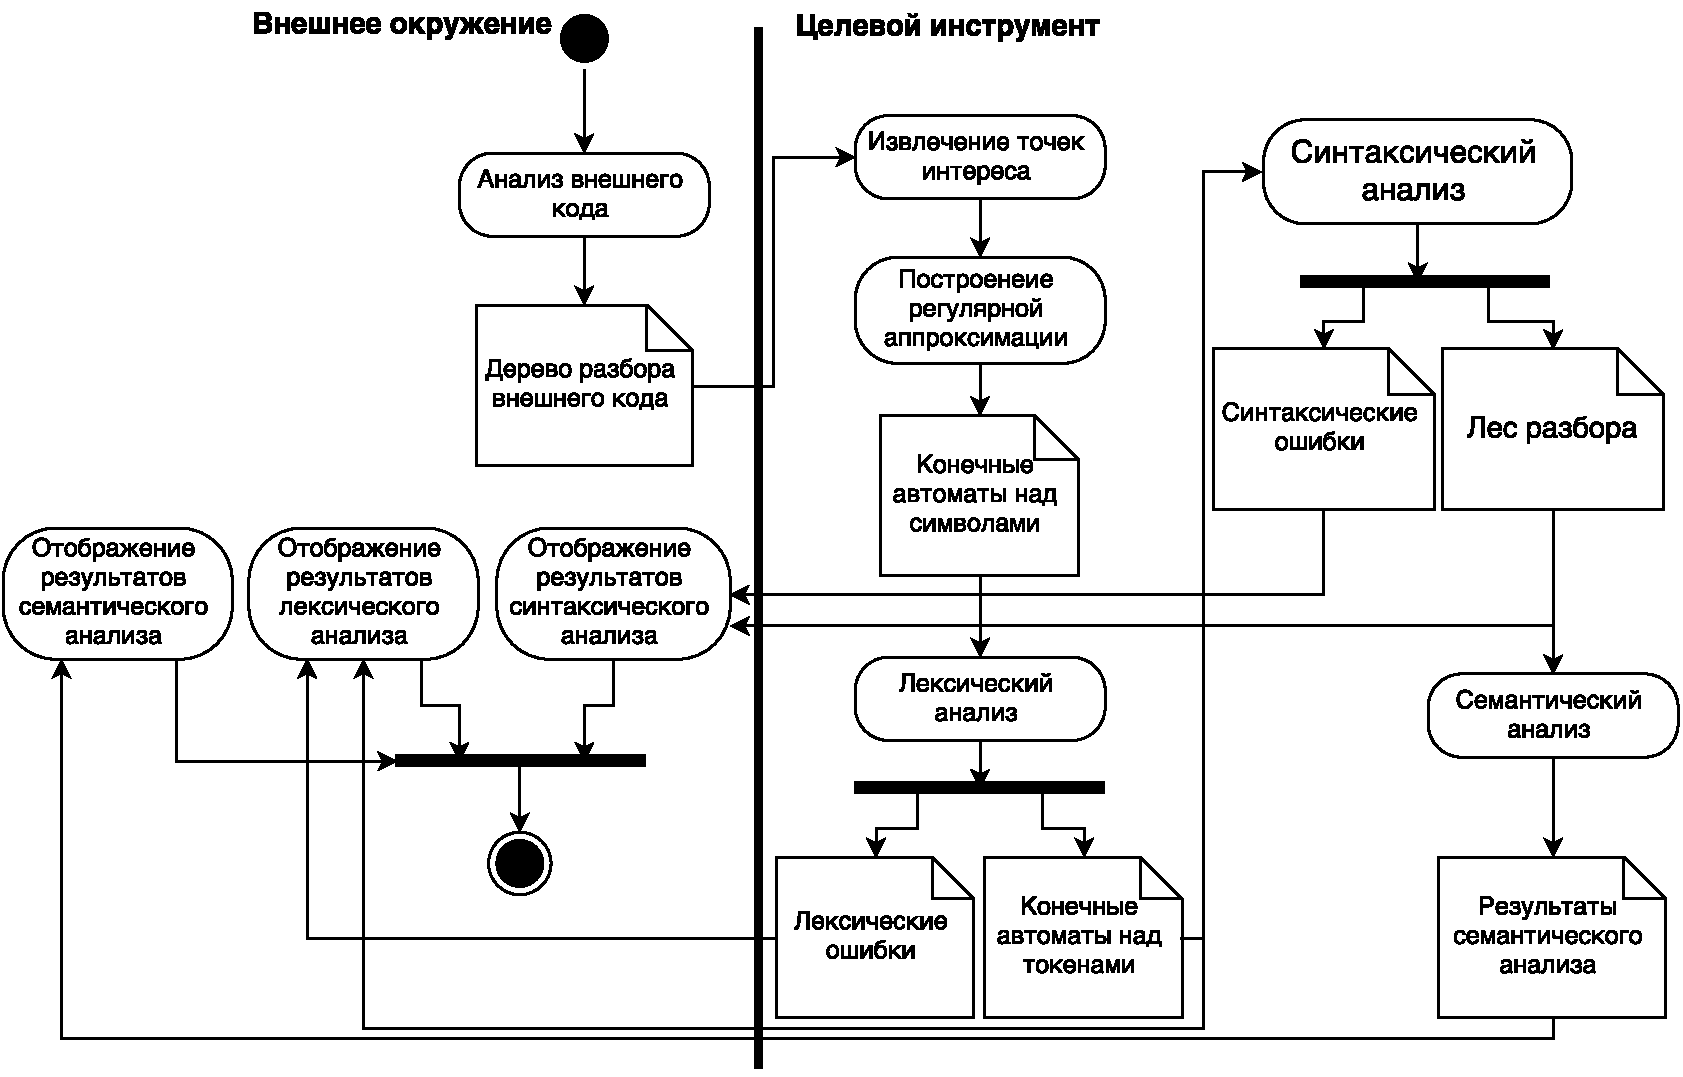
\includegraphics[width=0.8\textwidth]{pictures/Activ_SEL_Processing.pdf}
%   \end{center}
% \end{frame}

\begin{frame}
	\frametitle{Процесс работы(1/5)}
	% \textbf{Проектирование сервиса:}
	\begin{figure}[h]

	\centering
		
	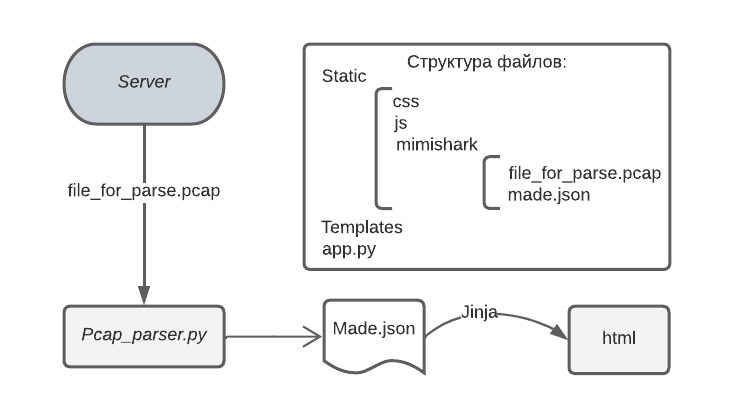
\includegraphics[width=0.8\linewidth]{Scheme_of_project.png}
		
	\caption{Схема обработки файлов на сервере}
		
	\label{fig:mpr}
		
\end{figure}
\end{frame}



\begin{frame}[fragile]{Процесс работы (2/5)}
% \textbf{Реализация серверной части:}
	% \lstset{numbers=left, numberstyle=\tiny, stepnumber=2, numbersep=5pt}
% 	\begin{lstlisting}[mathescape=true,caption=\textbf{Основной декоратор}, frame=single]
% @app.route( '/MimiShark' )
% 	def main_page( ):
% 	data = ReadJson(path)
% 	return render_template( 'main.html',pcap_data = data)		
%      \end{lstlisting}
% 	\begin{lstlisting}[mathescape=true,caption=\textbf{Основной декоратор, после внедрения}, frame=single]
% app.add_url_rule('/MimiShark',methods=['GET'], 
% 					view_func=mimishark_page)
% 	\end{lstlisting}
\begin{minipage}{5in}
		~~~~~~~~~~~~~~~~~~~~~~~~~~~~~~~~~~~~~~~~~~~\textbf{Основной декоратор}
\begin{Verbatim}[commandchars=\\\{\}]
	
	\textcolor{red}{@app.route}( '/MimiShark' )
	\textcolor{green}{def} main_page( ):
	\   \textcolor{blue}{data} = ReadJson(path)
	\   \textcolor{purple}{return} render_template( 'main.html',pcap_data = \textcolor{cyan}{data})
		
	
	
	\end{Verbatim}
	\end{minipage}	
\begin{minipage}{5in}
			~~~~~~~~~~~~~~~~~~~~~~~~~~~~~~~~~\textbf{Основной декоратор, после внедрения}
\begin{Verbatim}[commandchars=\\\{\}]
	
	\textcolor{red}{app}.add_url_rule('/MimiShark',methods=[\textcolor{green}{'GET'}], 
	\                                      view_func=\textcolor{cyan}{mimishark_page})
		
	\end{Verbatim}
		\end{minipage} 
\end{frame}
% Пришлось подстроиться под структуру файлов Miminet
% при этом vie_func = ссылается на ту же функцию из предыдущего листинга
% на сторону html передаем в качестве переменной pcap_data и с помощью шаблонизатора jinja выводим на странице

\begin{frame}[fragile]{Процесс работы (3/5)}
	% \textbf{Реализация графической составляющей:}
	% \lstset{numbers=left, numberstyle=\tiny, stepnumber=2, numbersep=5pt}
	\begin{figure}[h]

		\centering
			
		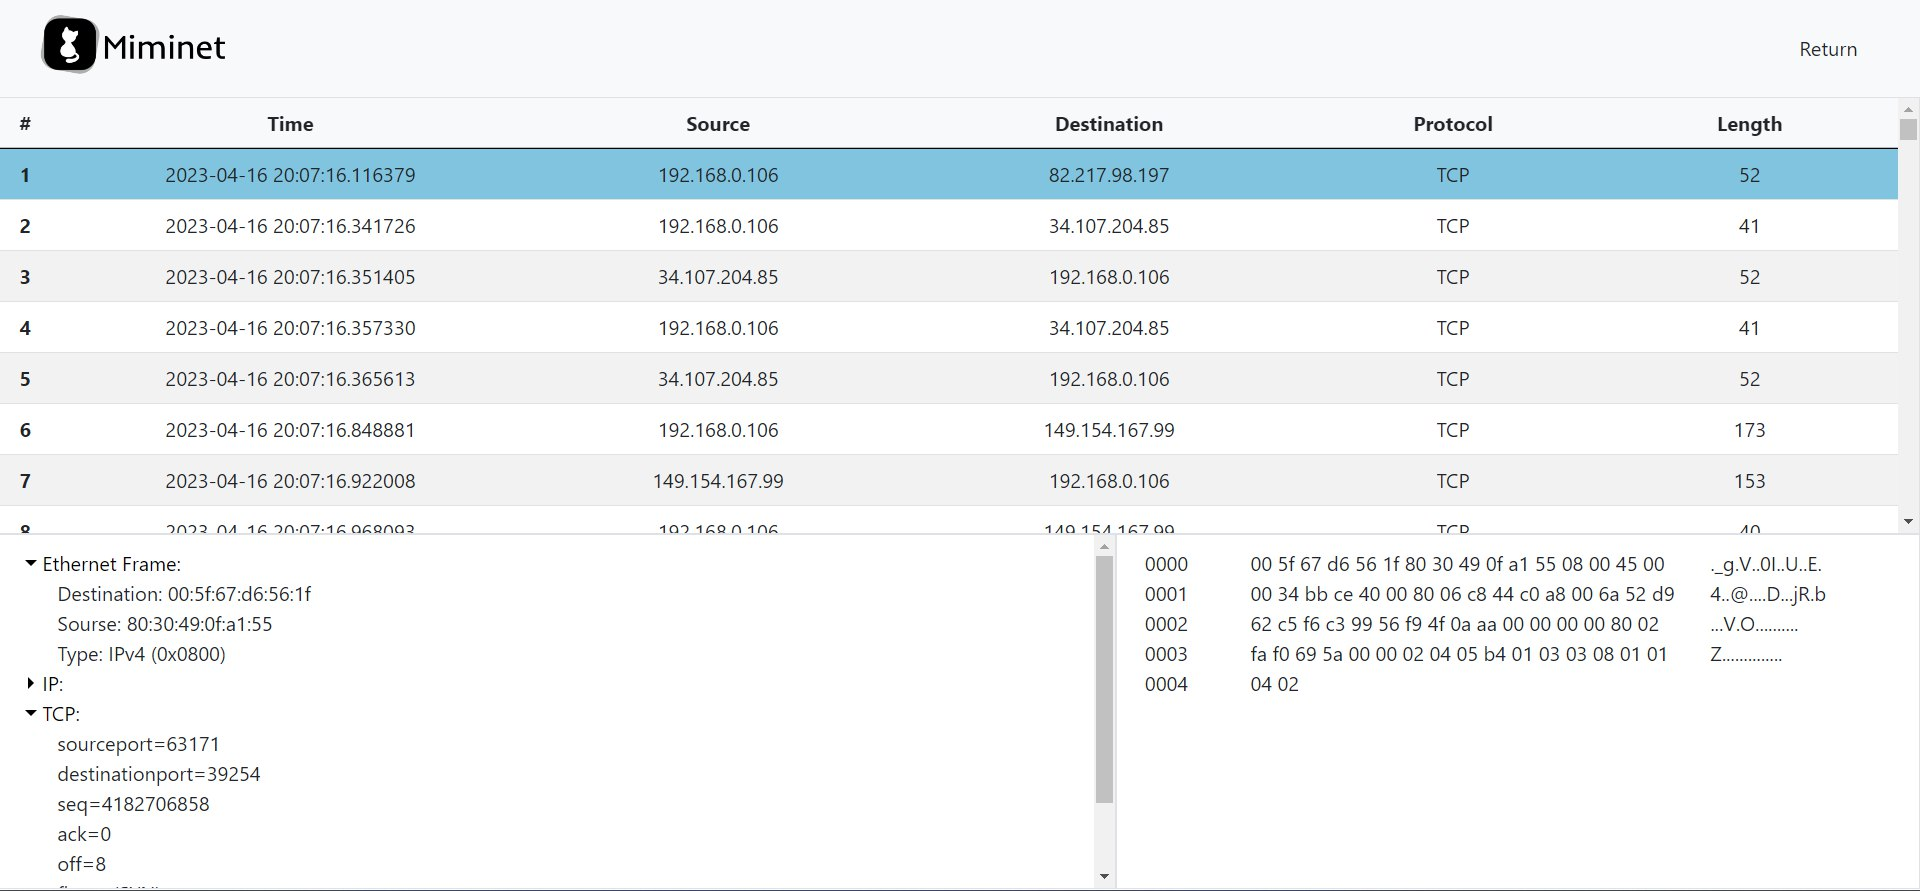
\includegraphics[width=0.8\linewidth]{cite.jpg}
			
		\caption{Внешний вид веб-страницы}
			
		\label{fig:mpr}
			
	\end{figure}
\end{frame}
% Помимо html и css был задействован javascript, с помощью которого  писались функции вывода данных о выбранном файле

\begin{frame}[fragile]{Процесс работы (4/5)}
	% \textbf{Парсинг и передача пакетов на сайт:}
	\begin{minipage}{5in}
		~~~~~~~~~~~~~~~~~~~~~~~~~~~~~~~~~\textbf{Работа парсера pcap файлов}
\begin{Verbatim}[commandchars=\\\{\}]

\ \textcolor{purple}{import} dpkt
\ \textcolor{green}{def} add_packets(pcap):
\   \textcolor{red}{for} timestamp, buf in pcap:
\      \textcolor{blue}{eth} = dpkt.ethernet.Ethernet(buf)
\      pcap_file[ "time" ] = str(datetime.datetime(timestamp))
\      \textcolor{blue}{ip} = eth.data
\	     pcap_file[ "source" ] = inet_to_str(ip.src)
\	     pcap_file[ "destination" ] = inet_to_str(ip.dst)
\	     pcap_file[ "protocol" ] = ip.get_proto(ip.p).__name__
\	     pcap_file[ "length" ] = ip.len
\	     ... 
	 \end{Verbatim}
	\end{minipage}
% 	\begin{lstlisting}[mathescape=true,caption=\textbf{Работа парсера pcap файлов}, frame=single]
% import dpkt
% def add_packets(pcap):
%   for timestamp, buf in pcap:
%    eth = dpkt.ethernet.Ethernet(buf)
%    pcap_file[ "time" ] = str(datetime.datetime(timestamp))
%    ip = eth.data
%    pcap_file[ "source" ] = inet_to_str(ip.src)
%    pcap_file[ "destination" ] = inet_to_str(ip.dst)
%    pcap_file[ "protocol" ] = ip.get_proto(ip.p).__name__
%    pcap_file[ "length" ] = ip.len
%    pcap_file[ "decode_ip" ] = ip_protocol_prop(ip)
%    pcap_file[ "bytes" ] = mac_to_str(buf)
%    pcap_file[ "ascii" ] = str(bytes.fromhex(i))[2:len((str(a)))-1] 
%    for i in bytes_repr
%      \end{lstlisting}
\end{frame}

% Существует также функция получения данных из протоколов, например для ip - это версия длина и тд.
% для tcp - флаги, sourseport, destinationport.

\begin{frame}[fragile]{Процесс работы (5/5)}
	\textbf{Внедрение готового проекта в Miminet:}
	% \lstset{numbers=left, numberstyle=\tiny, stepnumber=2, numbersep=5pt}
	\begin{figure}[h]

		\centering
			
		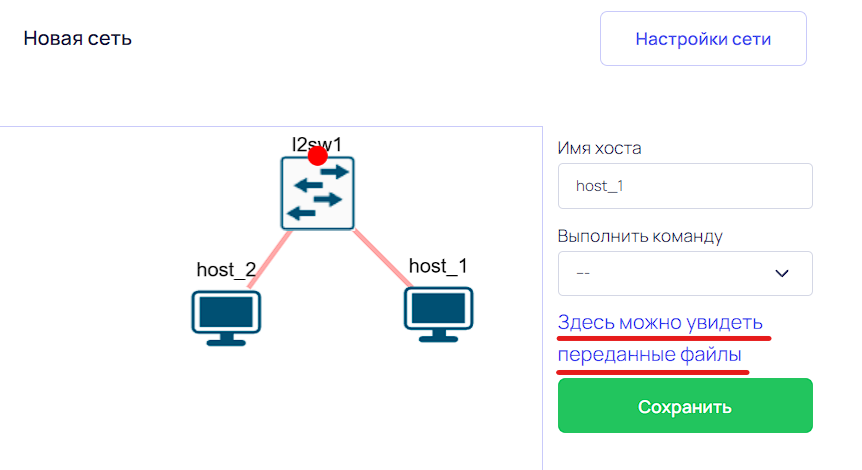
\includegraphics[width=0.6\linewidth]{Снимок экрана 2023-05-15 212721.png}
			
		\caption{Пример ссылки на анализатор в Miminet}
			
		\label{fig:mpr}
			
	\end{figure}
	Переход на страницу анализатора происходит по маршруту –
	/MimiShark?guid=...
\end{frame}

% \begin{frame}[t]
%   \frametitle{Экспериментальное исследование}
%   Постановка эксперимента
%   \begin{itemize}
%     \item На каком наборе данных проводилось экспериментальное исследование, почему были выбраны именно эти данные
%     \item На каком оборудовании проводилось исследование
%     \item Какие решения были выбраны для сравнения и почему
%   \end{itemize}
% \end{frame}
% \begin{frame}
% 	\frametitle{Тестирование}
% 	\begin{table}
% 		\caption{Замеры тестов для двух append$^o$}
% 		%\label{tabular}
% 		%\begin{center}
% 		\begin{tabular}{ccc}
% 			Длинна списка & Количество потоков & время, сек. \\%почему то при объединении не работает вовсе, можно попробовать работать с отдельно вызываемыми функциями
% 			7000          & 2                  & 26.7        \\
% 			7000          & 1                  & 27.5        \\
% 			8000          & 12                 & 24.2        \\
% 			8000          & 1                  & 40.4        \\
% 		\end{tabular}
% 		%\end{center}
% 	\end{table}

% 	\begin{block}{Вывод}
% 		После нескольких экспериментов сделан вывод, что запускать при малом количестве потоков, а также на малых обьемах данных не так выгодно, но при росте количества потоков пользы заметно больше.
% 	\end{block}

% \end{frame}

\begin{frame}
	\frametitle{Дальнейшие планы}
	\begin{itemize}
		\item Реализовать некоторые функции (фильтры поиска и т.д.)
		\item Добавить возможность импорта/экспорта данных
	\end{itemize}

\end{frame}

% \begin{frame}[t]
%   \frametitle{Результаты экспериментального исследования}
%   \begin{itemize}
%     \item Какие результаты показало экспериментальное исследование
%     \item Желательно привести графики, иллюстрирующие полученные результаты
%           \begin{itemize}
%             \item У иллюстраций должны быть подписи, у графиков --- легенда, подписи к осям, например:
%           \end{itemize}
%   \end{itemize}
%   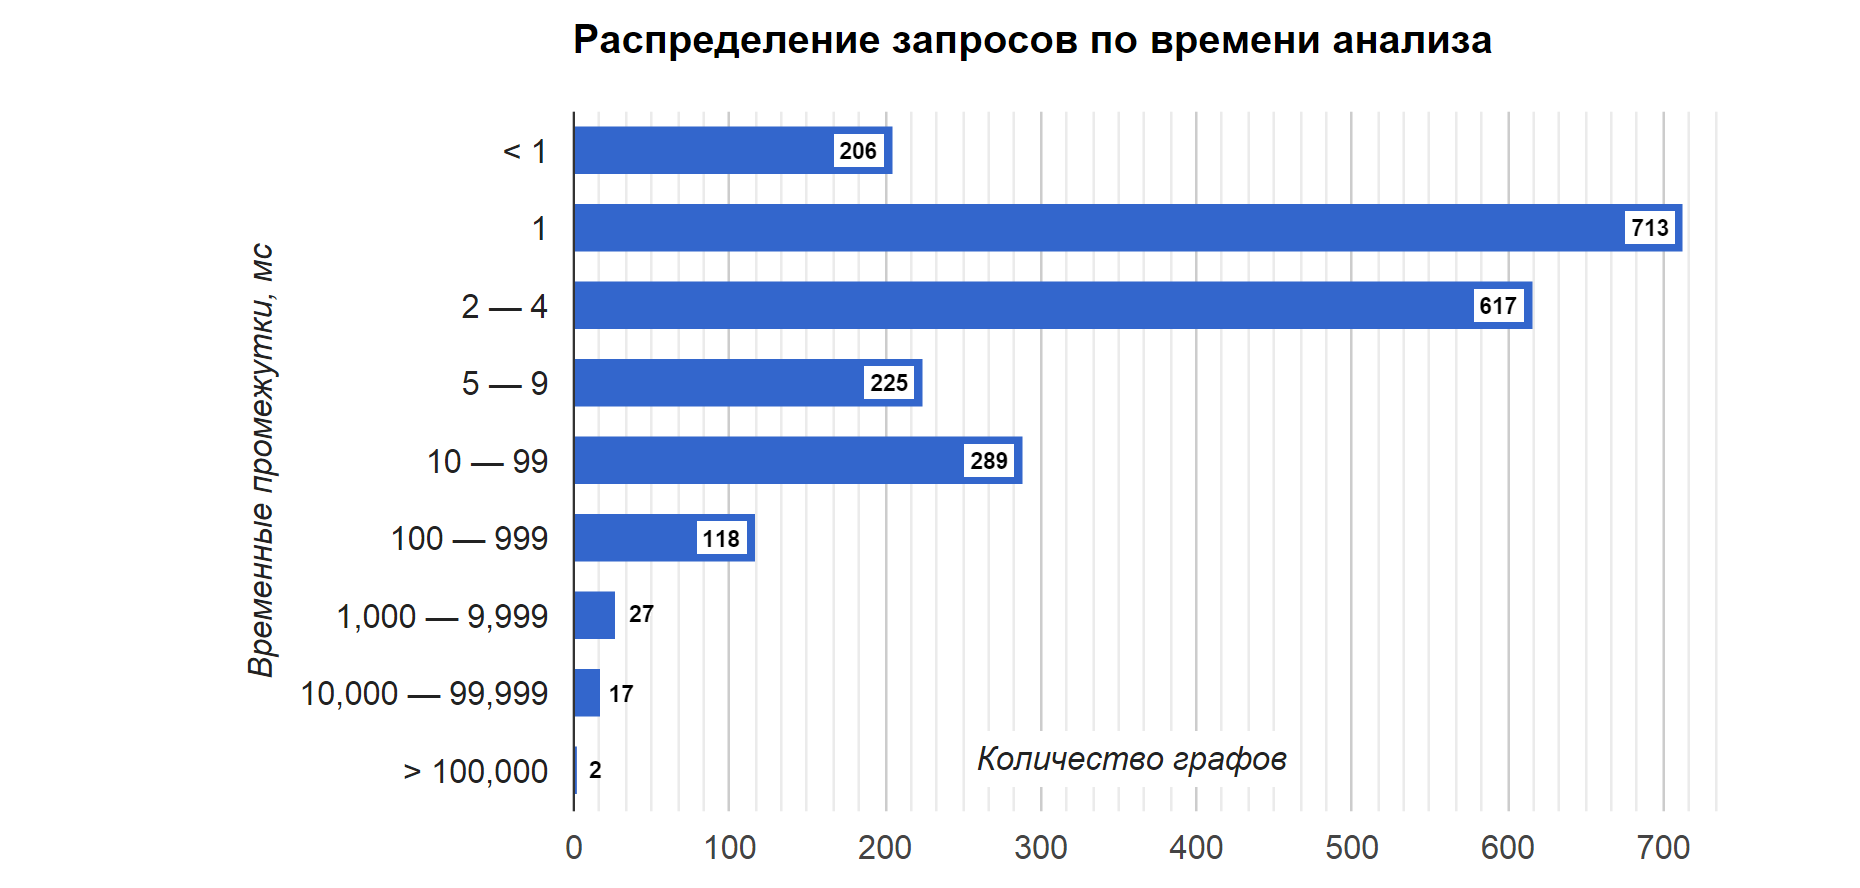
\includegraphics[width=10cm]{pictures/dist.png}
% \end{frame}


% \begin{frame}
%   \frametitle{Результаты}
%   \begin{itemize}
%     \item Практически то же, что и на слайде с постановкой задачи, но в совершенной форме --- что делал лично автор
%     \item Четкое отделение результатов своей работы (особенно для коллективных работ)
%     \item Формулировать глаголами совершенного вида в прошедшем времени (``сделано'', ``получено'')
%     \item Обсуждение (ограничения, валидность, альтернативы)
%     \item Не нужно слайдов типа ``Все'', ``Вопросы?'', ``Спасибо за внимание''
%   \end{itemize}

%   \begin{itemize}
%     \item Если результаты были представлены на конференции и опубликованы, это желательно указать
%   \end{itemize}
% \end{frame}

\begin{frame}
	\frametitle{Результаты}
	\begin{itemize}
		\item Проведен обзор веб-аналогов Wireshark
		      %\item Изучил примеры параллелизации
		      %\item Изучить примеры параллелизации
		\item Спроектирован сервис
		\item Написана веб-страница анализатора
		\item Информация о пакетах выведена на страницу
		\item Конечный продукт интегрирован в Miminet
	\end{itemize}

	\vspace{20mm}
	Всю проделанную работу можно посмотреть на github репозитории\footnote{\url{https://github.com/K0lba/MimiShark} (Дата доступа: 15.05.2023)}

	Версию, готовую для интеграции, можно посмотреть на github репозитории\footnote{\url{https://github.com/K0lba/NetFront} (Дата доступа: 30.05.2023)}

\end{frame}
% \begin{frame}[fragile]{Реализация альтернативного переключения состояния W\textasciicircum X [1/2]}
% 	\begin{minipage}{5in}
% 	~~~~~~~~~~~~~~~~~~~~~~~~~~~~~~~~~~~~~~~~~~~\textbf{Основной декоратор}
% 	\begin{Verbatim}[commandchars=\\\{\}]

% 	\textcolor{red}{@app.route}( '/MimiShark' )
% 	\textcolor{green}{def} main_page( ):
% 	\   \textcolor{blue}{data} = ReadJson(path)
% 	\   \textcolor{purple}{return} render_template( 'main.html',pcap_data = \textcolor{cyan}{data})
	


% \end{Verbatim}
% \end{minipage}	
% 	\begin{minipage}{5in}
% 		~~~~~~~~~~~~~~~~~~~~~~~~~~~~~~~~~\textbf{Основной декоратор, после внедрения}
% 		\begin{Verbatim}[commandchars=\\\{\}]

% 	\textcolor{red}{app}.add_url_rule('/MimiShark',methods=[\textcolor{green}{'GET'}], 
% 	\                                      view_func=\textcolor{cyan}{mimishark_page})
	
% 	 \end{Verbatim}
% 	\end{minipage} 
% 	% \begin{lstlisting}[mathescape=true,caption=\textbf{Основной декоратор}, frame=single]
% 	% 	@app.route( '/MimiShark' )
% 	% 		def main_page( ):
% 	% 		data = ReadJson(path)
% 	% 		return render_template( 'main.html',pcap_data = data)		
% 	% 		 \end{lstlisting}
% 	% 		\begin{lstlisting}[mathescape=true,caption=\textbf{Основной декоратор, после внедрения}, frame=single]
% 	% 	app.add_url_rule('/MimiShark',methods=['GET'], 
% 	% 						view_func=mimishark_page)
% 	% 		\end{lstlisting}
% \end{frame}

% \begin{frame}[fragile]{Реализация альтернативного переключения состояния W\textasciicircum X [1/2]}
% \begin{minipage}{5in}
% 		~~~~~~~~~~~~~~~~~~~~~~~~~~~~~~~~~\textbf{Работа парсера pcap файлов}
% \begin{Verbatim}[commandchars=\\\{\}]

% \ \textcolor{purple}{import} dpkt
% \ \textcolor{green}{def} add_packets(pcap):
% \   \textcolor{red}{for} timestamp, buf in pcap:
% \      \textcolor{blue}{eth} = dpkt.ethernet.Ethernet(buf)
% \      pcap_file[ "time" ] = str(datetime.datetime(timestamp))
% \      \textcolor{blue}{ip} = eth.data
% \	     pcap_file[ "source" ] = inet_to_str(ip.src)
% \	     pcap_file[ "destination" ] = inet_to_str(ip.dst)
% \	     pcap_file[ "protocol" ] = ip.get_proto(ip.p).__name__
% \	     pcap_file[ "length" ] = ip.len
% \	     ... 
% 	 \end{Verbatim}
% 	\end{minipage} 
% \end{frame}
%\addtocounter{framenumber}{1}
\appendix


\end{document}